\subsection{Десять проектов}

Проекты идут по возрастанию сложности: сначала последовательность команд и циклы, затем условия и датчики, потом полёт и камера, в конце нейросети и компьютерное зрение. У каждого есть снимок блоков, сгенерированный Python (тело программы, без импортов и \verb|finally|), разбор и результат. Готовые проекты лежат в \texttt{examples/python-onboard/bricks/}. Если не сказано иное, проект выполняется на земле, при выключенных двигателях.

\begin{center}\small
\begin{tabularx}{\linewidth}{@{}c>{\raggedright\arraybackslash}p{0.32\linewidth}>{\raggedright\arraybackslash}p{0.2\linewidth}X@{}}
\toprule
\textbf{№} & \textbf{Проект} & \textbf{Файл} & \textbf{Тема} \\
\midrule
1 & Светодиоды & \texttt{u01} & последовательность команд \\
2 & Бегущий огонь & \texttt{u02} & циклы, переменная-счётчик \\
3 & Телеметрия & \texttt{u03} & датчик и вывод данных \\
4 & Светофор высоты & \texttt{u04} & условия, бесконечный цикл \\
5 & Полёт по квадрату & \texttt{u05} & полётное задание (\textbf{полёт}) \\
6 & Фото под углами & \texttt{u06} & сервопривод, кадр, файл \\
7 & ИИ: люди & \texttt{u07} & детекция Yolo \\
8 & ИИ: жест & \texttt{u08} & поза YoloPose \\
9 & ИИ: текст & \texttt{u09} & PaddleOCR \\
10 & ArUco & \texttt{u10} & компьютерное зрение \\
\bottomrule
\end{tabularx}
\end{center}

\subsubsection*{Проект 1. Светодиоды: последовательность команд}

Блоки выполняются сверху вниз, один за другим. Это первая программа, цель --- увидеть, как цепочка блоков превращается в цепочку строк.

\begin{figure}[H]
\centering
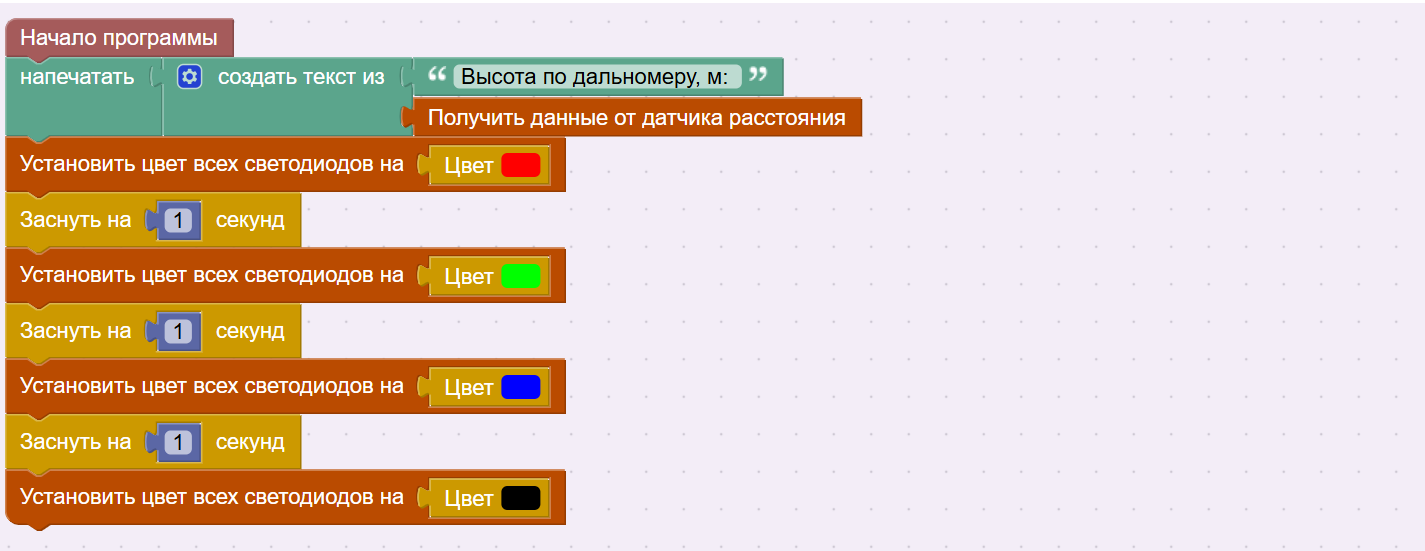
\includegraphics[width=0.62\textwidth]{images/bricks/blocks_u01_svetodiody.png}
\caption{Проект 1: светодиоды красным, зелёным, синим}
\end{figure}

\begin{codefile}[python]{python-onboard/bricks/python/u01_svetodiody.py}
\end{codefile}

\begin{itemize}
  \item Цвет задаётся блоком «Цвет» из категории «Прочее»; Bricks переводит его из вида \texttt{\#RRGGBB} в доли 0..1 для \verb|led_control|. Чёрный цвет --- светодиоды выключены.
  \item «Заснуть на 1 секунд» --- пауза: без неё смена цветов была бы незаметна.
  \item Первый блок «напечатать высоту» нужен из-за особенности Bricks 2.3.0 (раздел~\ref{sec:bricks-limits}): без блока, читающего данные дрона, в программу не попадает строка \verb|pioneer = Pioneer()|.
\end{itemize}

\expected{светодиоды по секунде горят красным, зелёным и синим, затем гаснут.}

\subsubsection*{Проект 2. Бегущий огонь: циклы и переменная-счётчик}

\begin{figure}[H]
\centering
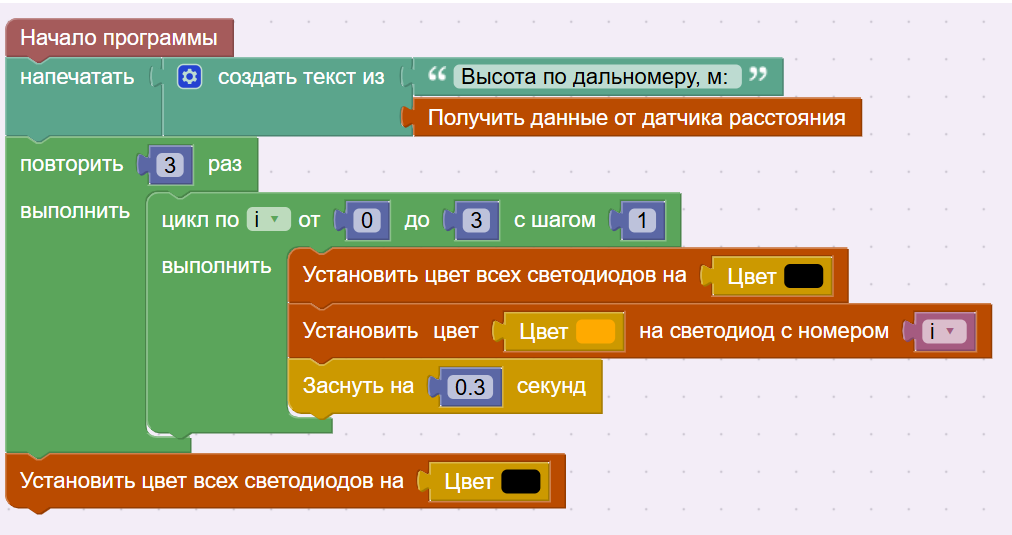
\includegraphics[width=0.72\textwidth]{images/bricks/blocks_u02_beguschiy_ogon.png}
\caption{Проект 2: огонь бежит по четырём светодиодам}
\end{figure}

\begin{codefile}[python]{python-onboard/bricks/python/u02_beguschiy_ogon.py}
\end{codefile}

\begin{itemize}
  \item «повторить 3 раз» --- внешний цикл: огонь пробегает три круга.
  \item «цикл по \texttt{i} от 0 до 3 с шагом 1» --- внутренний цикл; \texttt{i} принимает значения 0, 1, 2, 3 и служит номером светодиода. Bricks превратил его в \verb|range(0, 4)|: граница «до 3» включается.
  \item Перед каждым включением все светодиоды гасятся, поэтому горит ровно один.
\end{itemize}

\begin{taskbox}[Огонь в обратную сторону]
Пустите огонь от 3 до 0 с шагом $-1$. Затем добавьте второй, «догоняющий» огонь другого цвета на светодиоде с номером \texttt{(i + 2) \% 4}.
\expected{по кругу бегут два огонька разных цветов, расстояние между ними не меняется.}
\end{taskbox}

\subsubsection*{Проект 3. Телеметрия: вывод данных}

\begin{figure}[H]
\centering
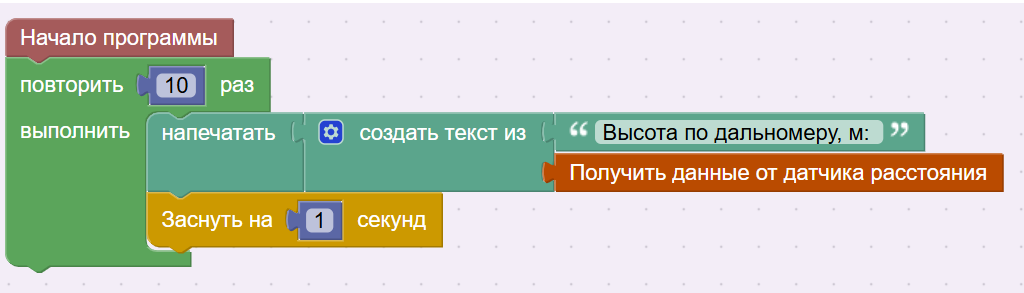
\includegraphics[width=0.75\textwidth]{images/bricks/blocks_u03_telemetriya.png}
\caption{Проект 3: десять измерений высоты}
\end{figure}

\begin{codefile}[python]{python-onboard/bricks/python/u03_telemetriya.py}
\end{codefile}

\begin{itemize}
  \item «создать текст из» склеивает подпись и число; Bricks сам добавил \verb|str(...)|, чтобы склеить строку с числом.
  \item 10 повторений с паузой в секунду --- десять измерений за десять секунд.
\end{itemize}

\expected{в панели «Вывод программы» десять строк «Высота по дальномеру, м: …». Поднимите дрон рукой (при выключенных двигателях!) --- значение изменится.}

\subsubsection*{Проект 4. Светофор высоты: условия}

\begin{figure}[H]
\centering
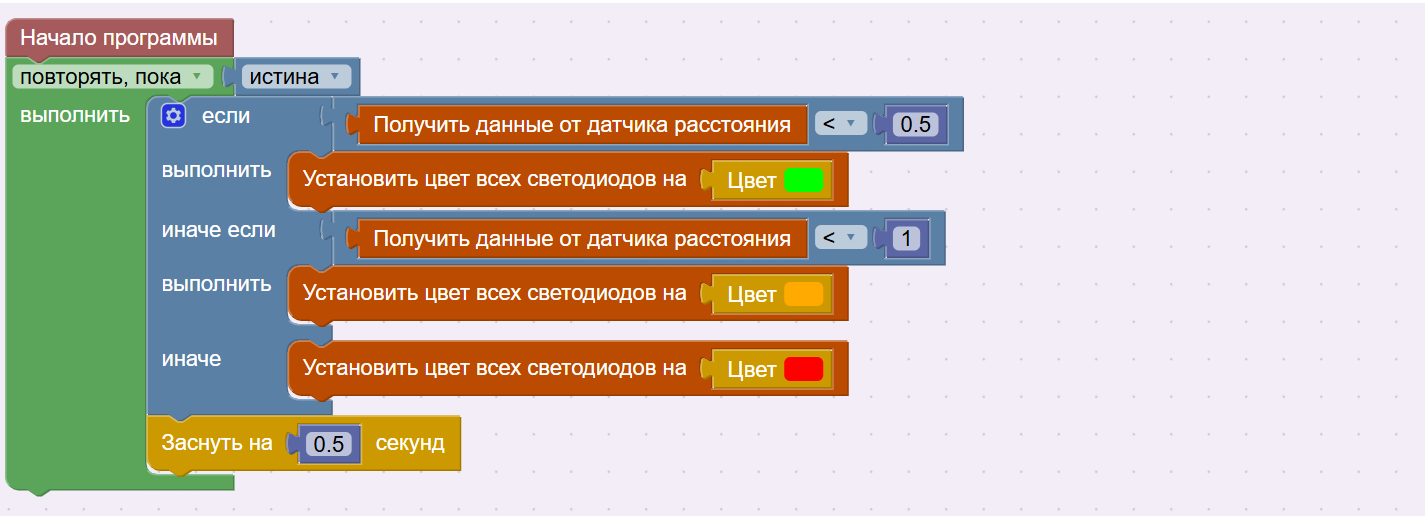
\includegraphics[width=0.72\textwidth]{images/bricks/blocks_u04_svetofor_vysoty.png}
\caption{Проект 4: цвет светодиодов зависит от высоты}
\end{figure}

\begin{codefile}[python]{python-onboard/bricks/python/u04_svetofor_vysoty.py}
\end{codefile}

\begin{itemize}
  \item Ветки проверяются по порядку: ниже 0.5~м --- зелёный; иначе ниже 1~м --- жёлтый; во всех остальных случаях --- красный.
  \item Шестерёнка на блоке «если» добавляет ветки «иначе если» и «иначе».
  \item «повторять, пока истина» --- бесконечный цикл; программа работает до нажатия \ui{Стоп}. Здесь сказывается безопасное завершение: после остановки выполнится \verb|finally|.
\end{itemize}

\begin{taskbox}[Свой светофор]
Добавьте четвёртый уровень: выше 2~м светодиоды мигают красным. Подсказка: понадобится ещё одна ветка «иначе если» и пауза внутри неё.
\expected{при подъёме дрона рукой цвет последовательно меняется зелёный, жёлтый, красный, мигающий красный.}
\end{taskbox}

\subsubsection*{Проект 5. Полёт по квадрату}

\begin{alertbox}[Этот проект поднимает дрон в воздух]
Запускайте его только на подготовленной площадке $2\times2$~м с пультом в руках. При подготовке главы эта программа на дроне \textbf{не запускалась}: показаны только блоки и сгенерированный код. Запускайте сначала с одним отрезком пути.
\end{alertbox}

\begin{figure}[H]
\centering
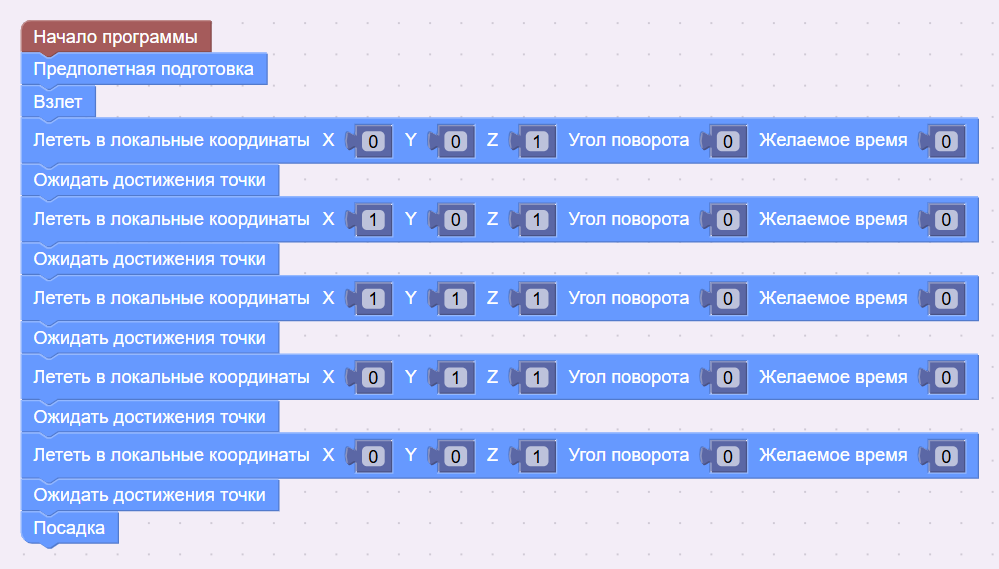
\includegraphics[width=0.85\textwidth]{images/bricks/blocks_u05_polet_kvadrat.png}
\caption{Проект 5: взлёт, четыре точки квадрата, посадка}
\end{figure}

\begin{codefile}[python]{python-onboard/bricks/python/u05_polet_kvadrat.py}
\end{codefile}

\begin{itemize}
  \item «Лететь в локальные координаты» \emph{не ждёт} прилёта, поэтому после каждого полёта стоит «Ожидать достижения точки». Без него дрон сразу получит следующую команду и «срежет» угол квадрата.
  \item Это та же программа, что полёт по квадрату в главе~\ref{sec:sdk2}, только собранная из блоков.
\end{itemize}

\subsubsection*{Проект 6. Фото под разными углами камеры}

\begin{figure}[H]
\centering
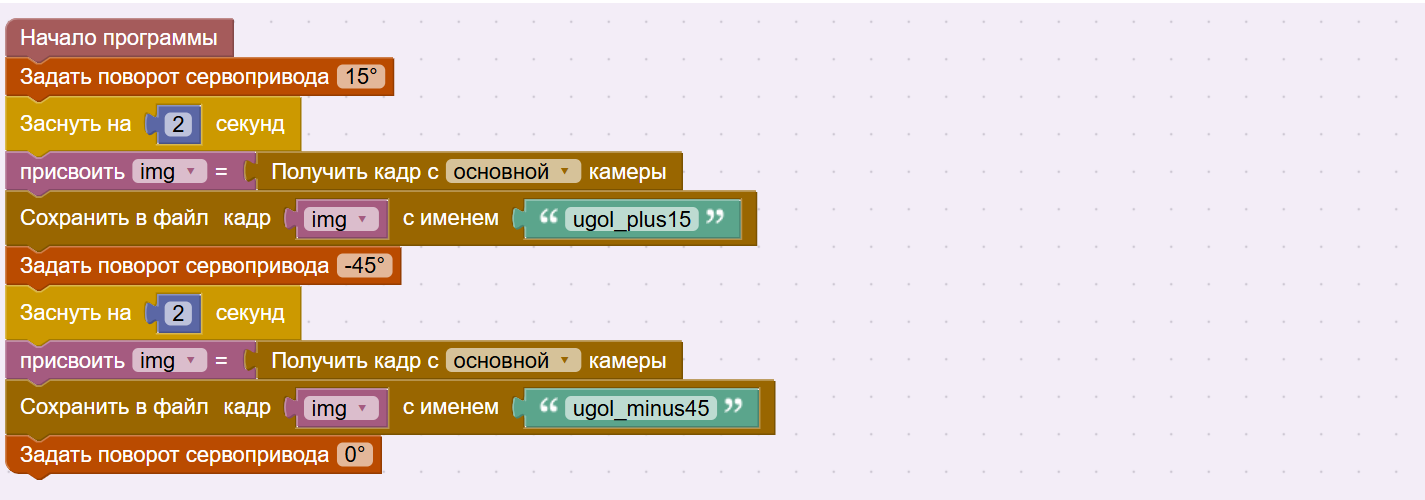
\includegraphics[width=0.6\textwidth]{images/bricks/blocks_u06_foto_ugly.png}
\caption{Проект 6: наклон камеры, кадр, сохранение}
\end{figure}

\begin{codefile}[python]{python-onboard/bricks/python/u06_foto_ugly.py}
\end{codefile}

\begin{itemize}
  \item «Задать поворот сервопривода» --- угол выбирается на циферблате с шагом $15^\circ$ в диапазоне от $-80^\circ$ до $+30^\circ$. Если вписать 20, Bricks округлит до 15 (раздел~\ref{sec:bricks-limits}).
  \item «Сохранить в файл кадр с именем» пишет снимок в \texttt{/mnt/media/photos/<имя>.jpg}: фото сразу видны в «Галерее медиа» Pioneer Code.
  \item Пауза в 2~секунды после поворота нужна, чтобы камера успела повернуться и снимок не смазался.
\end{itemize}

\begin{taskbox}[Фото-серия]
Снимите четыре кадра с углами $0^\circ$, $-30^\circ$, $-60^\circ$, $-75^\circ$ и именами, по которым видно угол. Используйте цикл с переменной или четыре повтора.
\expected{в галерее четыре фото с понятными именами; при большем наклоне в кадре больше пола.}
\end{taskbox}

\subsubsection*{Нейросети и компьютерное зрение}

Блоки ИИ работают так же, как классы \verb|Yolo|, \verb|YoloPose| и \verb|PaddleOCR| из главы~\ref{sec:rknn}: сначала блок «Инициализация ИИ модели» загружает модель на NPU, затем в цикле кадр камеры передаётся модели. Результат удобно смотреть в окне: блок «Демонстрация изображения из кадра … в окно \emph{имя}» публикует кадр, окно открывается по адресу \texttt{http://10.42.0.1:8889/<имя>/}. Проекты 7--10 проверены запуском сгенерированного кода на дроне.

\subsubsection*{Проект 7. Найти людей}

\begin{figure}[H]
\centering
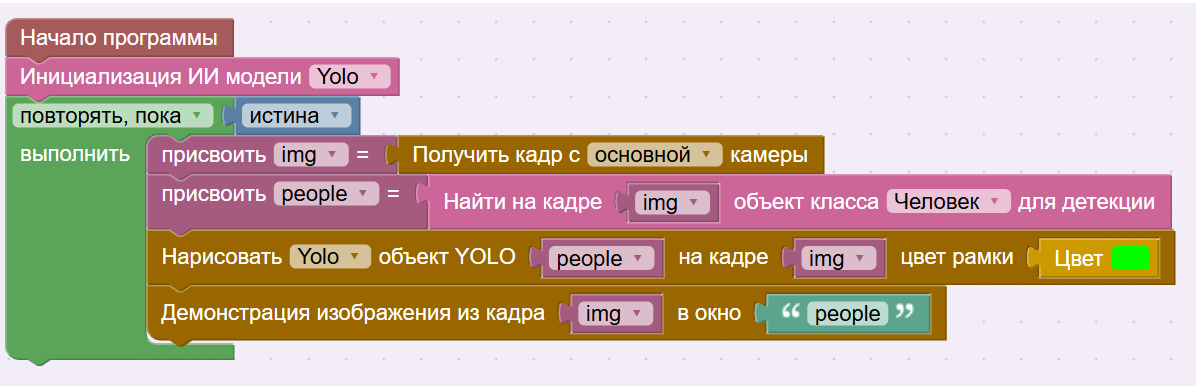
\includegraphics[width=0.95\textwidth]{images/bricks/blocks_u07_ii_lyudi.png}
\caption{Проект 7: детекция людей и рамки на кадре}
\end{figure}

\begin{codefile}[python]{python-onboard/bricks/python/u07_ii_lyudi.py}
\end{codefile}

\begin{itemize}
  \item «Найти на кадре \texttt{img} объект класса Человек» --- детекция с фильтром по классу (в списке 80 классов COCO по-русски). Результат сохраняется в переменную \texttt{people}.
  \item «Нарисовать Yolo объект \texttt{people} на кадре \texttt{img}» рисует рамки, «Демонстрация…» отправляет кадр в окно \texttt{people}.
  \item Bricks сам добавил кэш \verb|infer_cache_per_frame|: если на одном кадре нейросеть вызывается несколько раз, она считает его один раз.
\end{itemize}

\begin{figure}[H]
\centering
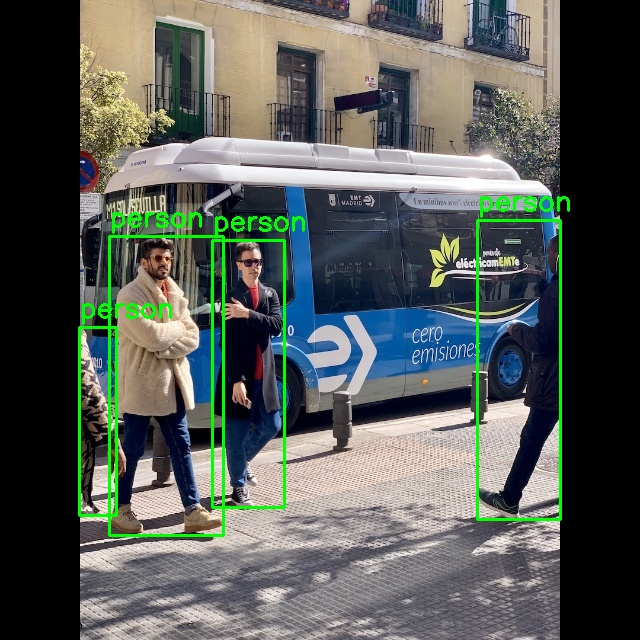
\includegraphics[width=0.45\textwidth]{images/bricks/br07_people_2.jpg}
\caption{Результат проекта 7 на дроне (на вход подано тестовое изображение): рамки вокруг людей, автобус не выделен --- работает фильтр «Человек»}\label{fig:bricks-people}
\end{figure}

\expected{окно \texttt{http://10.42.0.1:8889/people/} с рамками вокруг людей; на дроне программа обрабатывала около 7--8 кадров в секунду.}

\subsubsection*{Проект 8. Жест «две руки вверх» включает свет}

\begin{figure}[H]
\centering
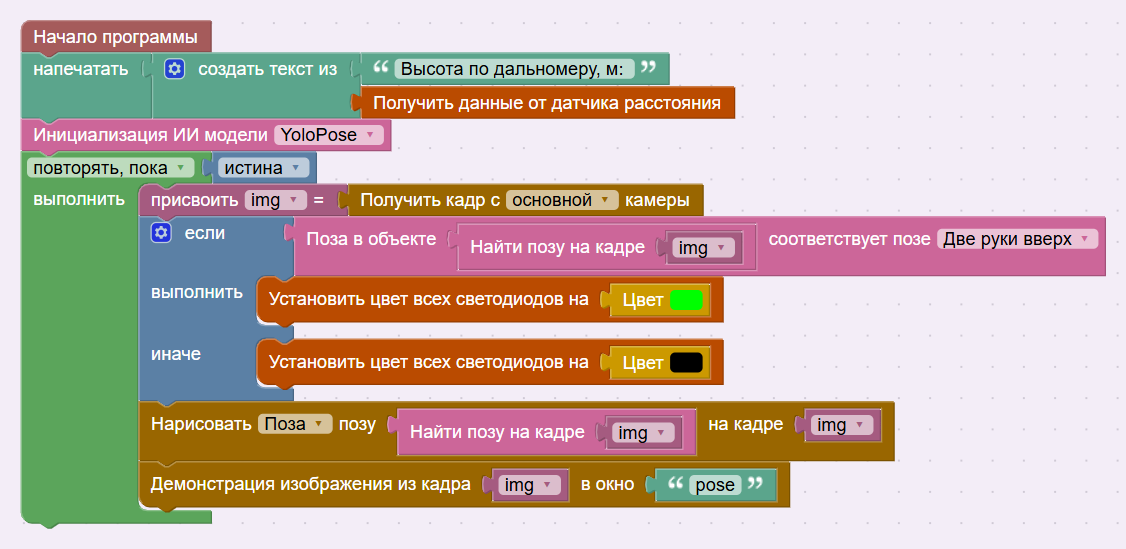
\includegraphics[width=0.9\textwidth]{images/bricks/blocks_u08_ii_zhest.png}
\caption{Проект 8: поза человека управляет светодиодами}
\end{figure}

\begin{codefile}[python]{python-onboard/bricks/python/u08_ii_zhest.py}
\end{codefile}

\begin{itemize}
  \item «Поза в объекте … соответствует позе Две руки вверх» возвращает «истину», только если жест держится несколько кадров подряд (параметр \verb|THRESHOLD| в сгенерированном коде). Это защита от случайных срабатываний: тот же приём устойчивого решения по нескольким кадрам вы встретили в главе~\ref{sec:rknn}.
  \item Доступные позы: левая и правая рука вверх или в сторону, две руки вверх, обе в стороны, кисти рядом в центре.
  \item «Нарисовать Позу» рисует скелет на кадре, окно называется \texttt{pose}.
\end{itemize}

\expected{поднимите обе руки --- через несколько кадров светодиоды загорятся зелёным; опустите --- погаснут.}

\subsubsection*{Проект 9. Распознать текст}

\begin{figure}[H]
\centering
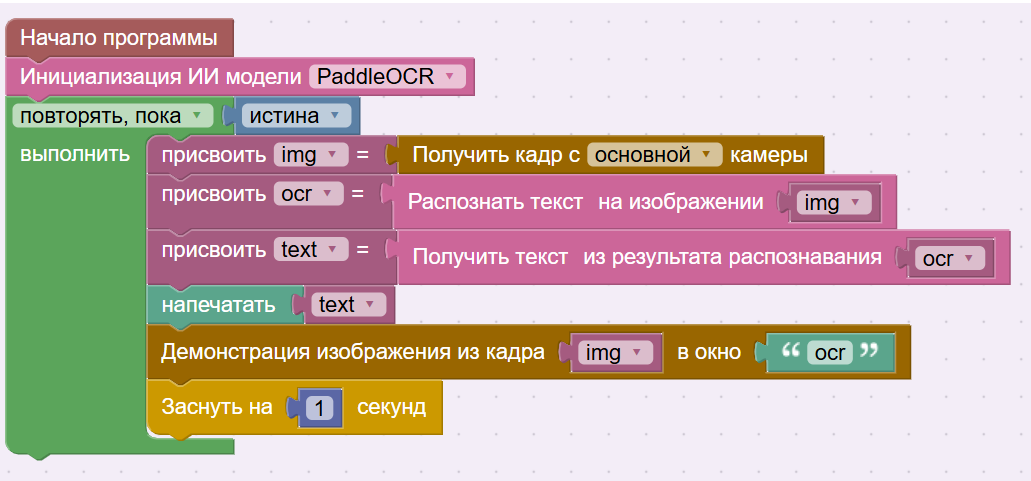
\includegraphics[width=0.78\textwidth]{images/bricks/blocks_u09_ii_tekst.png}
\caption{Проект 9: распознавание текста PaddleOCR}
\end{figure}

\begin{codefile}[python]{python-onboard/bricks/python/u09_ii_tekst.py}
\end{codefile}

\begin{itemize}
  \item Результат распознавания сначала сохраняется в переменную \texttt{ocr}, и только потом из него извлекается текст. Если вложить блоки друг в друга напрямую, Bricks~2.3.0 сгенерирует код с синтаксической ошибкой (раздел~\ref{sec:bricks-limits}).
  \item «Заснуть на 1 секунд»: распознавание тяжёлое, чаще раза в секунду оно обычно и не нужно.
\end{itemize}

\begin{figure}[H]
\centering
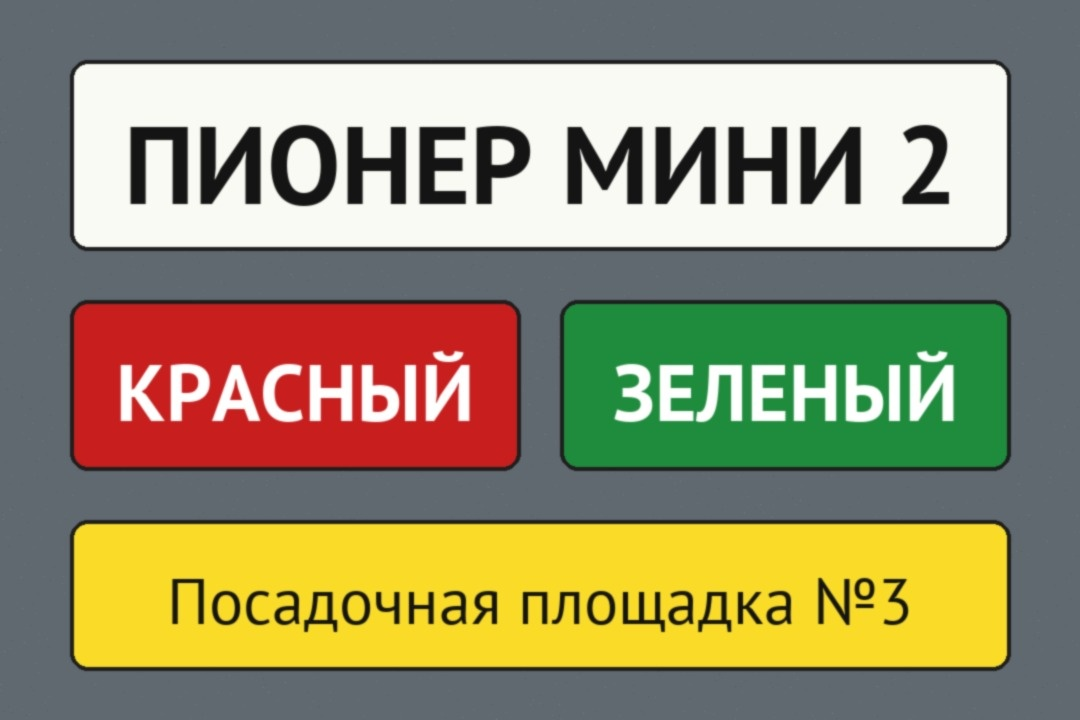
\includegraphics[width=0.6\textwidth]{images/bricks/br09_ocr_2.jpg}
\caption{Окно \texttt{ocr} программы на дроне (на вход подана табличка с текстом)}\label{fig:bricks-ocr}
\end{figure}

Вывод программы на дроне для таблички с рис.~\ref{fig:bricks-ocr}:

\begin{verbatim}
ПИОНЕР МИНИ2
КРАCНЬИ
зеленый
Посадочная площадка
\end{verbatim}

В слове «КРАCНЬИ» вторая буква~С латинская: модель смешивает похожие буквы двух алфавитов, поэтому результат сравнивают по смыслу, а не посимвольно.

\begin{infobox}[Окно ocr появляется не сразу]
Распознавание медленное, да ещё в цикле стоит пауза в секунду: в окно уходит меньше одного кадра в секунду. Поэтому окно \texttt{http://10.42.0.1:8889/ocr/} начинает показывать видео только через 20--30 секунд после запуска --- браузер ждёт первого полного (ключевого) кадра. Уберите блок «Заснуть», если нужно более живое изображение.
\end{infobox}

\subsubsection*{Проект 10. Маркеры ArUco}

\begin{figure}[H]
\centering
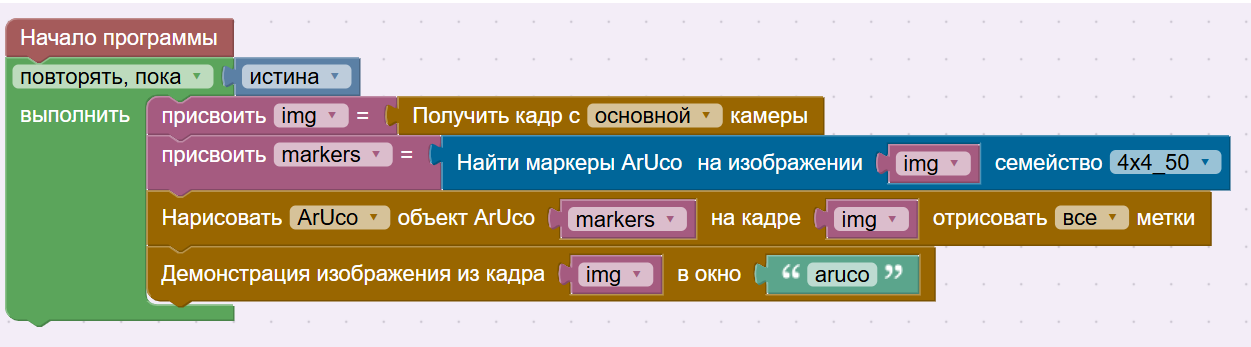
\includegraphics[width=0.95\textwidth]{images/bricks/blocks_u10_aruco.png}
\caption{Проект 10: поиск и отрисовка маркеров ArUco}
\end{figure}

\begin{codefile}[python]{python-onboard/bricks/python/u10_aruco.py}
\end{codefile}

\begin{itemize}
  \item «Найти маркеры ArUco на изображении \texttt{img} семейство 4x4\_50» --- семейство должно совпадать с напечатанными маркерами.
  \item Блоки «Координаты объекта» и «Размер объекта» из «Компьютерного зрения» дают центр и размер маркера с нужным ID --- с ними можно, например, поворачивать дрон к маркеру.
\end{itemize}

\expected{в окне \texttt{http://10.42.0.1:8889/aruco/} найденные маркеры обведены и подписаны номерами; на дроне программа работала с частотой около 7 кадров в секунду.}

\begin{taskbox}[Маркер в центре]
Выведите в «Вывод программы» координаты центра маркера с ID~0. Включайте зелёный свет, когда маркер находится в центральной трети кадра, и красный --- когда нет.
\expected{при смещении маркера в кадре цвет светодиодов меняется на границах центральной трети; координаты в выводе согласованы с положением маркера.}
\end{taskbox}
